\section{Model}\label{a:model}
%===================================================================================================
\subsection{Structure \& Notation}\label{a:model.struc}
Table~\ref{tab:strata} summarizes the modelled population stratifications,
including 2~sex $\times$ 4~activity $\times$ (\,5~HIV $\times$ 5~cascade $+$ 1~susceptible)
= 208 total possible states.
Figure~\ref{fig:model} summarizes the model structure and state transitions with respect to
(\subref{fig:model.risk}) risk groups and partnership types;
(\subref{fig:model.hiv}) HIV status; and
(\subref{fig:model.care}) ART cascade.
\begin{table}[h]
  \centering
  \caption{Modelled stratifications: population (top) and partnership-level dimensions (bottom)}
  \begin{tabular}{lccl}
  \toprule
  Stratification & \multicolumn{2}{c}{Index} & Strata          \\
  \midrule
  \textbf{Sex}               & $s$ & 1 & Heterosexual Women    \\
                             &     & 2 & Heterosexual Men      \\[1ex]
  \textbf{Activity group}    & $i$ & 1 & Lower Activity        \\
                             &     & 2 & Medium Activity       \\
                             &     & 3 & Lower Risk Sex Work   \\
                             &     & 4 & Higher Risk Sex Work  \\[1ex]
  \textbf{HIV status}        & $h$ & 1 & Susceptible           \\
                             &     & 2 & Acute HIV             \\
                             &     & 3 & CD4 $>$ 500           \\
                             &     & 4 & 350 $<$ CD4 $<$ 500   \\
                             &     & 5 & 200 $<$ CD4 $<$ 350   \\
                             &     & 6 & CD4 $<$ 200 (AIDS)    \\[1ex]
  \textbf{ART cascade}       & $c$ & 1 & Undiagnosed           \\
                             &     & 2 & Diagnosed \& Linked   \\
                             &     & 3 & Diagnosed \& Unlinked \\
                             &     & 4 & On ART                \\
                             &     & 5 & Virally Suppressed    \\
  \midrule
  \textbf{Partnership types} & $p$ & 1 & Main / Spousal        \\
                             &     & 2 & Casual                \\
                             &     & 3 & Occasional Sex Work   \\
                             &     & 4 & Regular Sex Work      \\[1ex]
  \textbf{Sex act types}     & $a$ & 1 & Vaginal               \\
                             &     & 2 & Anal                  \\
  \bottomrule
\end{tabular}
  \label{tab:strata}
\end{table}
\begin{figure}[h]
  \begin{subfigure}{\linewidth}
    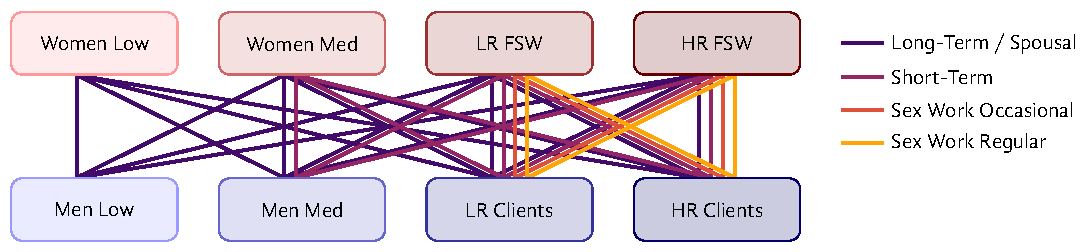
\includegraphics[scale=.72]{model.risk}
    \caption{Risk groups and partnership types}
    \label{fig:model.risk}
  \end{subfigure}
  \begin{subfigure}{\linewidth}
    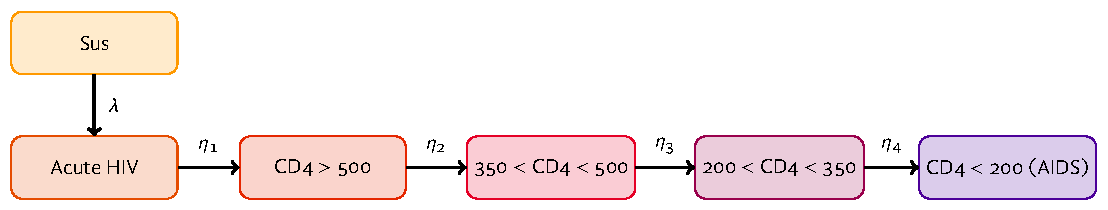
\includegraphics[scale=.72]{model.hiv}
    \caption{HIV states}
    \label{fig:model.hiv}
  \end{subfigure}
  \begin{subfigure}{\linewidth}
    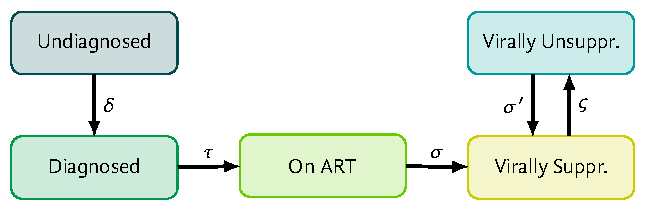
\includegraphics[scale=.72]{model.cascade}
    \caption{ART cascade states}
    \label{fig:model.care}
  \end{subfigure}
  \caption{Model structure and transitions}
  \label{fig:model}
  \floatfoot{Notation ---
    Low/LR: lower risk; Med: medium risk; HR: higher risk; FSW: female sex workers; Clients: of FSW;
    CD4: CD4+ T-cell count per mm\tsup{3};
    Not shown: turnover amongst risk groups in (\subref{fig:model.risk}).}
\end{figure}
%===================================================================================================
\subsection{Parameterization}\label{a:model.param}
\clearpage
%===================================================================================================
\subsection{Calibration}\label{a:model.cal}
Figures~\ref{fig:fit.prev}~and~\ref{fig:fit.inc} illustrate HIV prevalence and incidence
in the base case scenario, and the associated calibration targets.
Figure~\ref{fig:fit.pr} similarly shows prevalence ratios between selected risk groups.
\begin{figure}[h]
    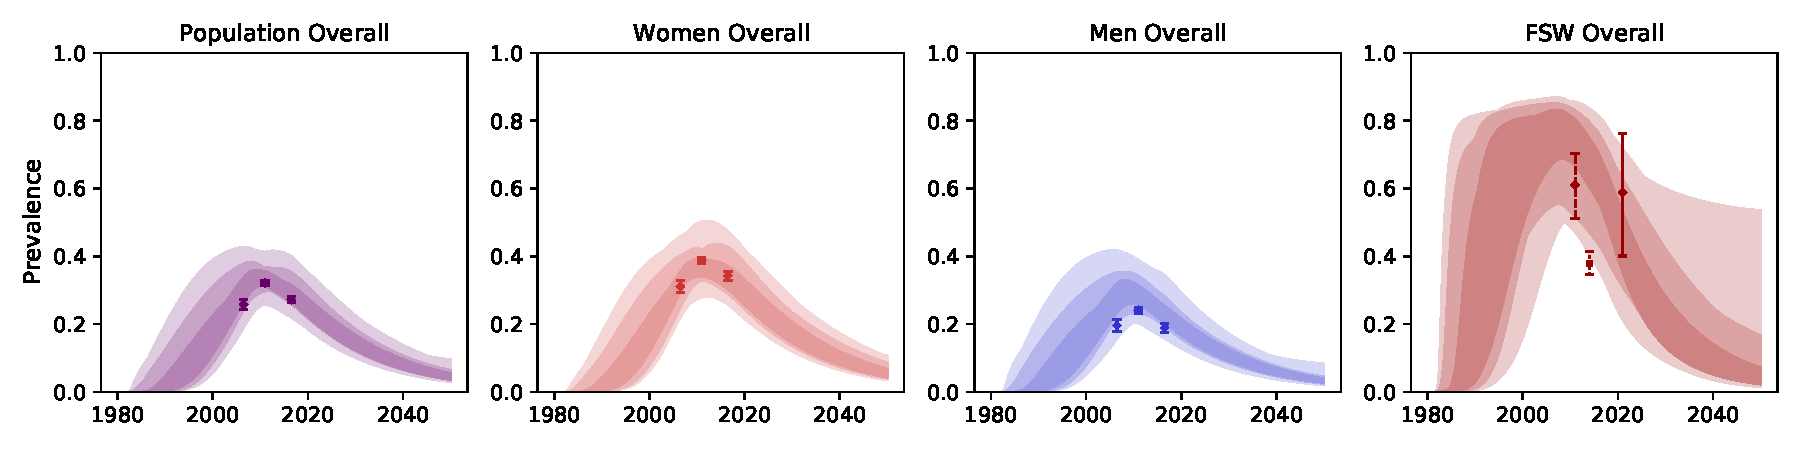
\includegraphics[width=\linewidth]{fit-prev}
  \caption{HIV prevalence in the base case scenario and associated calibration targets}
  \label{fig:fit.prev}
  \floatfoot{Three ribbons illustrate range of 100\%, top 20\%, and top 4\% of model fits
    by likelihood for all base case calibration targets;
    points and error bars illustrate the mean and 95\% CI for each calibration target.}
\end{figure}
\begin{figure}[h]
    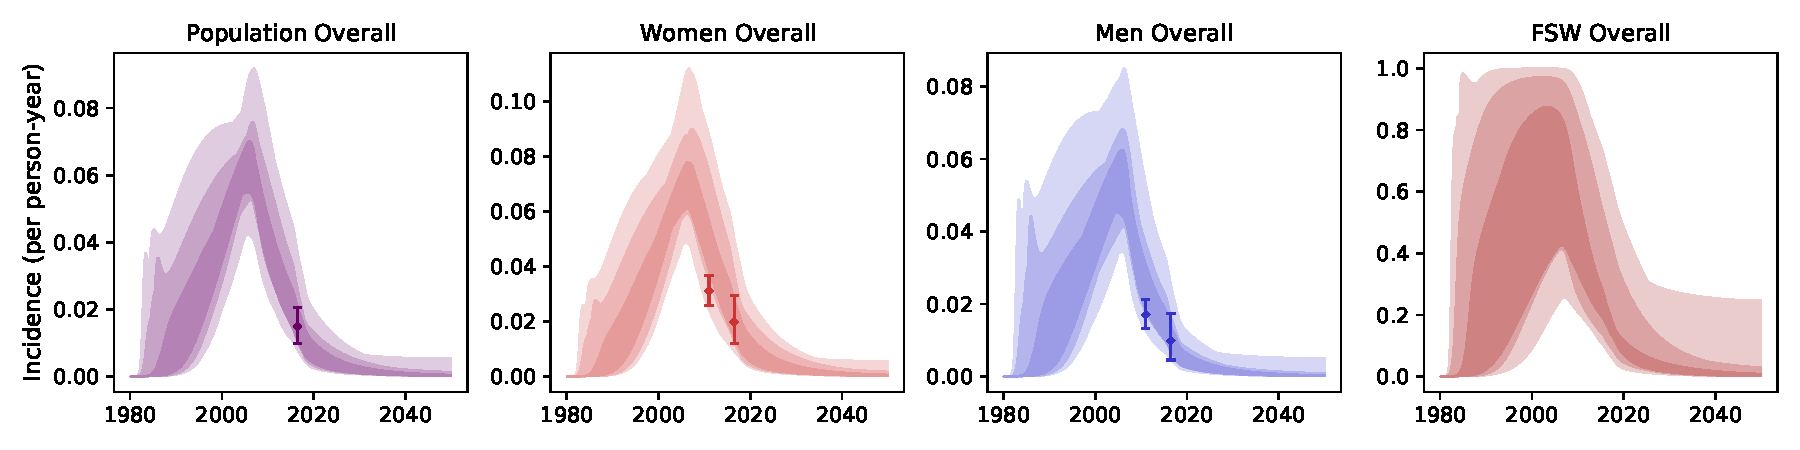
\includegraphics[width=\linewidth]{fit-inc}
  \caption{HIV incidence in the base case scenario and associated calibration targets}
  \label{fig:fit.inc}
  \floatfoot{Three ribbons illustrate range of 100\%, top 20\%, and top 4\% of model fits
    by likelihood for all base case calibration targets;
    points and error bars illustrate the mean and 95\% CI for each calibration target.}
\end{figure}
\begin{figure}[h]
  % TODO: wrap this like facet & deal with long titles
  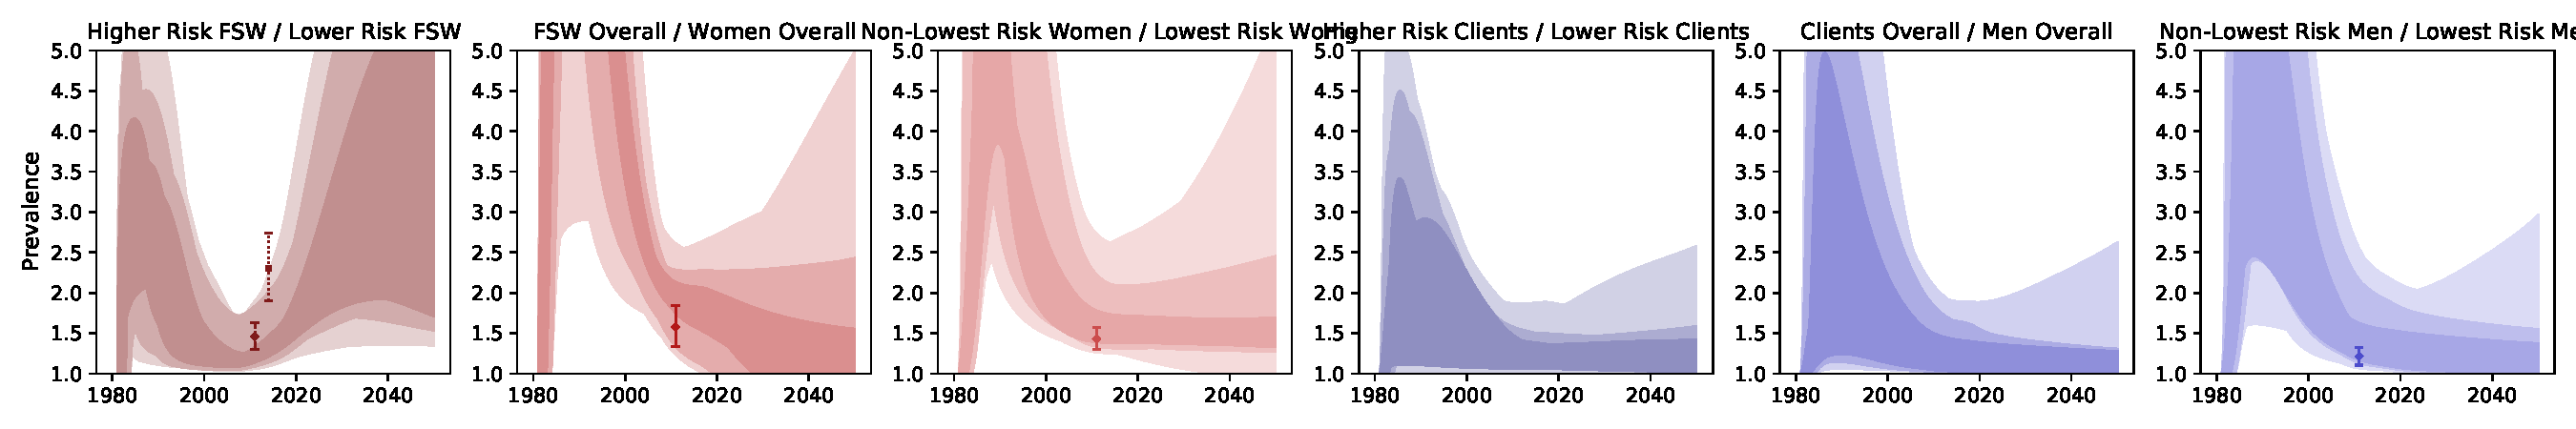
\includegraphics[width=\linewidth]{fit-pr}
  \caption{HIV prevalence ratios in the base case scenario and associated calibration targets}
  \label{fig:fit.pr}
  \floatfoot{Three ribbons illustrate range of 100\%, top 20\%, and top 4\% of model fits
    by likelihood for all base case calibration targets;
    points and error bars illustrate the mean and 95\% CI for each calibration target.}
\end{figure}
\clearpage\newgeometry{top=1cm,bottom=2cm}
\begin{figure}[h]
  \begin{subfigure}{\linewidth}
    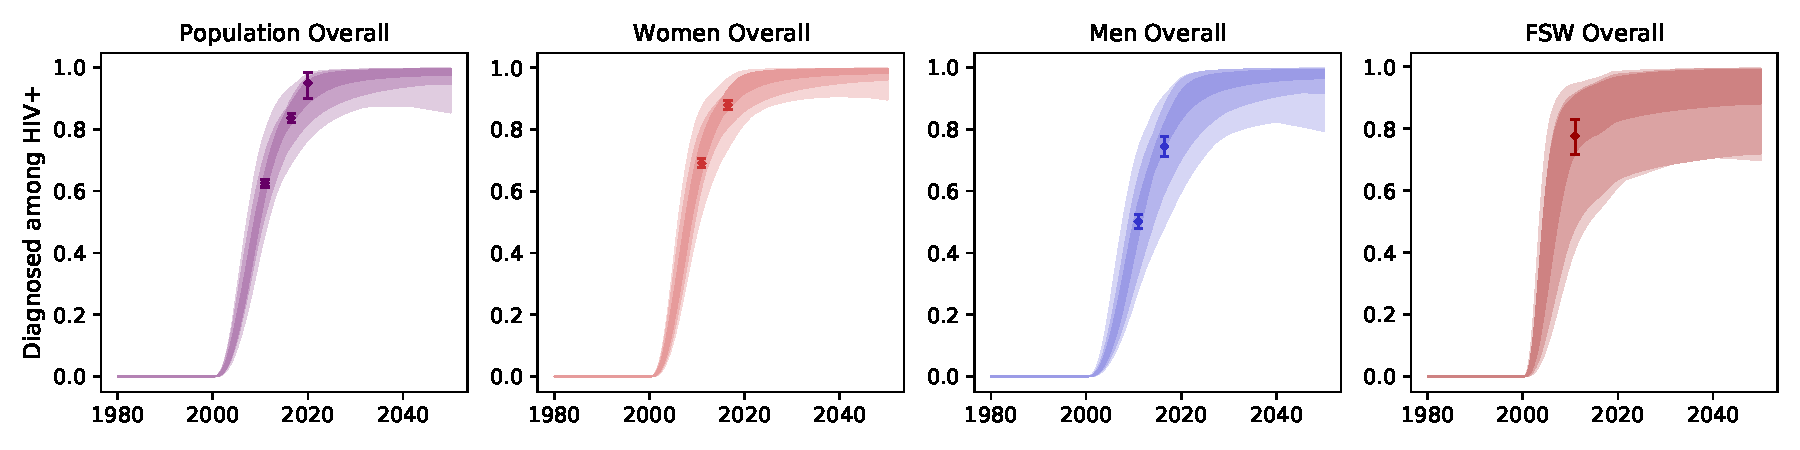
\includegraphics[width=\linewidth]{fit-diag}
    \caption{\% Diagnosed among HIV+}
    \label{fig:fit.cas.dx}
  \end{subfigure}
  \begin{subfigure}{\linewidth}
    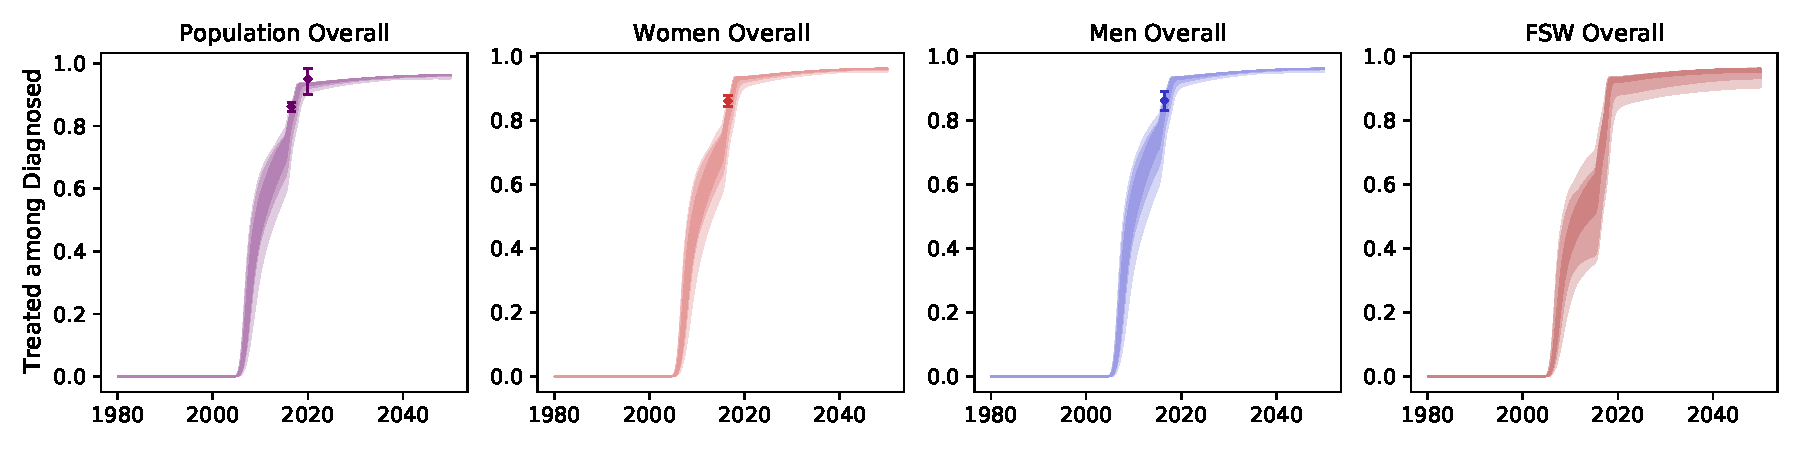
\includegraphics[width=\linewidth]{fit-treat-c}
    \caption{\% On ART among diagnosed}
    \label{fig:fit.cas.treat-c}
  \end{subfigure}
  \begin{subfigure}{\linewidth}
    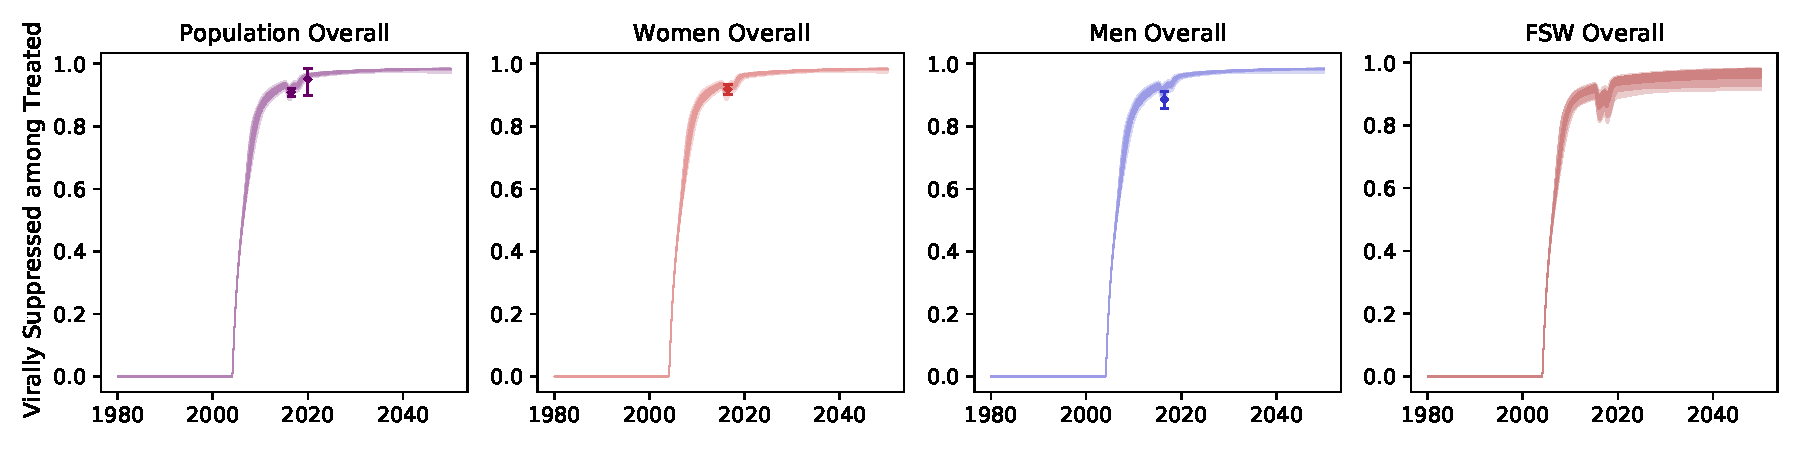
\includegraphics[width=\linewidth]{fit-vls-c}
    \caption{\% Virally suppressed among on ART}
    \label{fig:fit.cas.vls-c}
  \end{subfigure}
  \begin{subfigure}{\linewidth}
    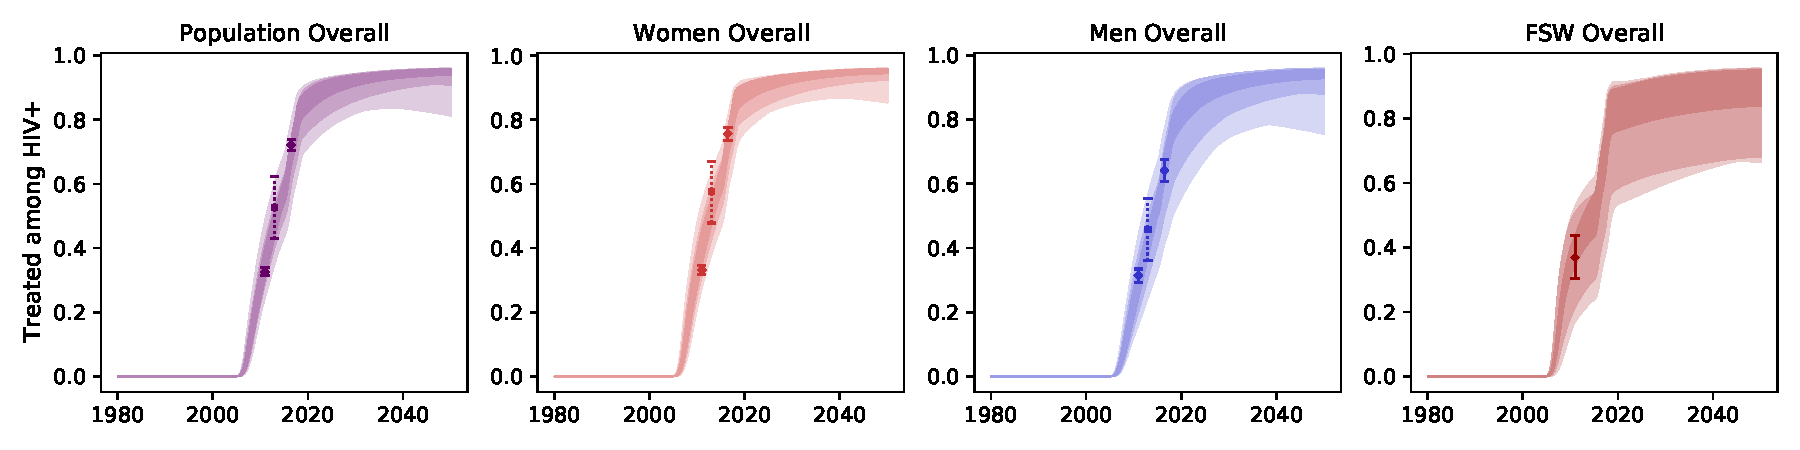
\includegraphics[width=\linewidth]{fit-treat-u}
    \caption{\% On ART among HIV+}
    \label{fig:fit.cas.treat-u}
  \end{subfigure}
  \begin{subfigure}{\linewidth}
    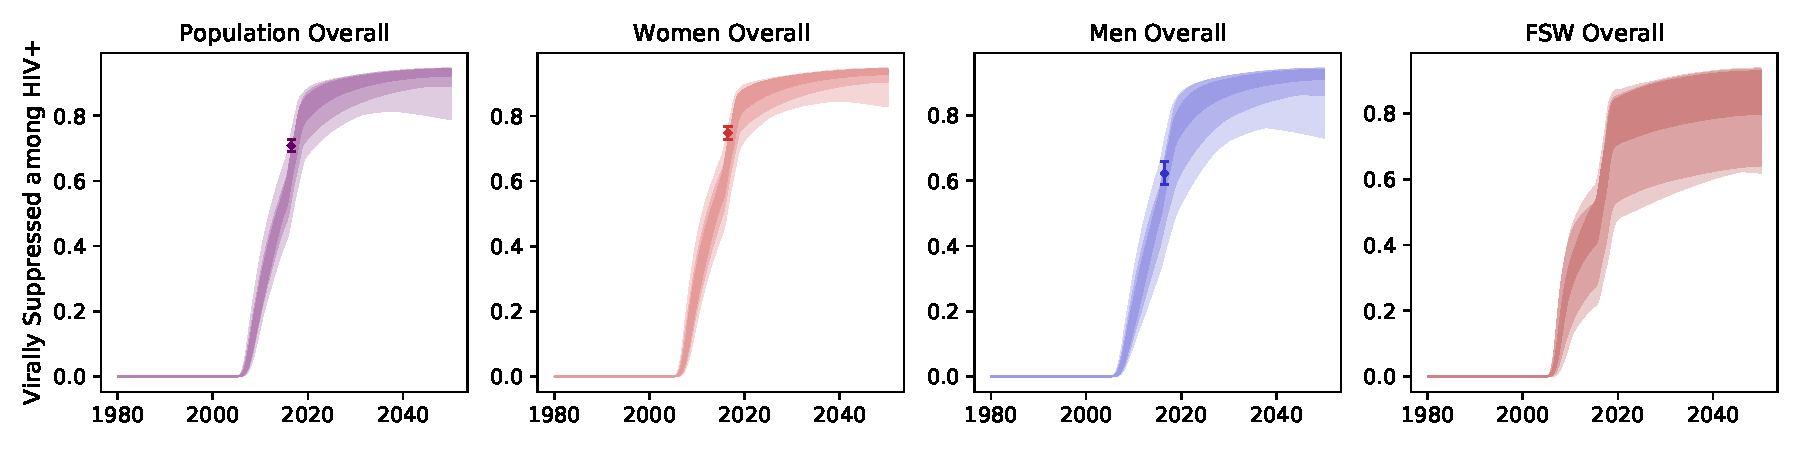
\includegraphics[width=\linewidth]{fit-vls-u}
    \caption{\% Virally suppressed HIV+}
    \label{fig:fit.cas.vls-u}
  \end{subfigure}
  \caption{ART cascade in the base case scenario and associated calibration targets}
  \label{fig:fit.cas}
  \floatfoot{Three ribbons illustrate range of 100\%, top 20\%, and top 4\% of model fits
    by likelihood for all base case calibration targets;
    points and error bars illustrate the mean and 95\% CI for each calibration target.}
\end{figure}
\clearpage\restoregeometry
\begin{figure}[h]
  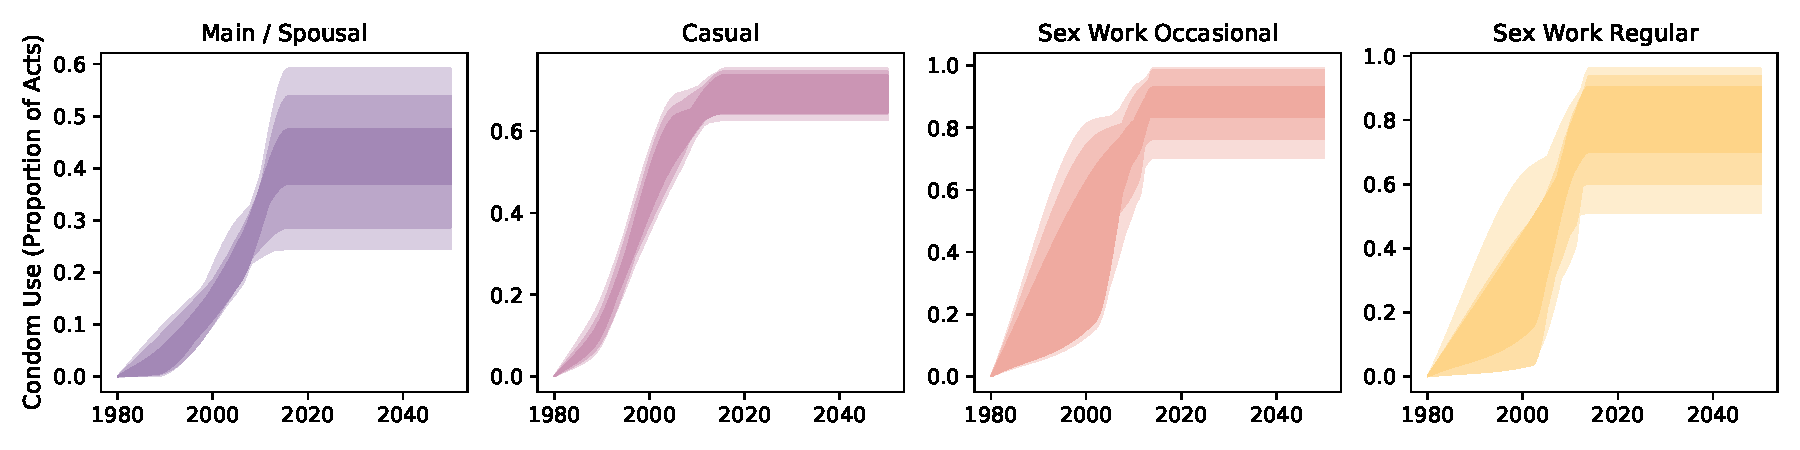
\includegraphics[width=\linewidth]{fit-condom}
  \caption{Condom use by partnership type in the base case scenario and associated calibration targets}
  \label{fig:fit.condom}
  \floatfoot{Three ribbons illustrate range of 100\%, top 20\%, and top 4\% of model fits
    by likelihood for all base case calibration targets}
%    points and error bars illustrate the mean and 95\% CI for each calibration target.}
  % TODO: plot condom use "targets" with weights = 0 ?
\end{figure}
\clearpage
\printbibliography